\chapter{振动和波 光 相对论(选修3-4)}

\section{机械振动}


1.简谐运动

(1)定义:物体在跟位移大小成正比并且总是指向\_\_平衡位置\_\_的回复力作用下的振动.

(2)平衡位置:物体在振动过程中\_\_回复力\_\_为零的位置.

(3)回复力

\ding{172}定义:使物体返回到\_\_平衡位置\_\_的力.

\ding{173}方向:总是指向\_\_平衡位置\_\_.

\ding{174}来源:属于\_\_效果\_\_力,可以是某一个力,也可以是几个力的\_\_合力\_\_或某个力的\_\_分力\_\_.

(4)简谐运动的两种模型

\ding{172}弹簧振子

\ding{173}单摆

2.简谐运动的公式和图象

(1)简谐运动的表达式

\ding{172}动力学表达式:F=\_\_-kx\_\_,其中``-''表示回复力与位移的方向相反.

\ding{173}运动学表达式:x=!!! Asin($\omega t+\varphi$) \#\#\#,其中A代表振幅,$\omega$=2πf表示简谐运动的快慢,($\omega t+\varphi$)代表简谐运动的相位,$\varphi$叫做\_\_初相\_\_.

(2)简谐运动的图象

\ding{172}从\_\_平衡位置\_\_开始计时,函数表达式为x=Asin $\omega$t,图象如图甲所示.

\ding{173}从\_\_最大位移\_\_处开始计时,函数表达式为x=Acos $\omega$t,图象如图乙所示.

\begin{center}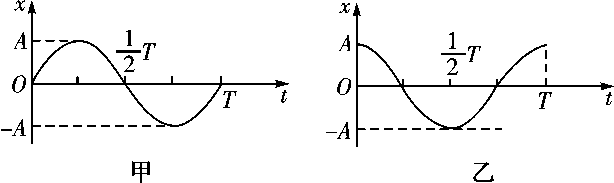
\includegraphics[width=2.79236in,height=0.82986in]{media/image511.png}\end{center}
3.简谐运动的运动规律

(1)对称规律

\ding{172}做简谐运动的物体,在关于平衡位置对称的两点,回复力、位移、加速度具有等大反向的关系.另外,速度的大小、动能具有\_\_对称性\_\_,速度的方向可能\_\_相同\_\_或\_\_相反\_\_.

\ding{173}振动物体来回通过相同的两点间的时间相等,如tBC=tCB;振动物体经过关于平衡位置对称的等长的两线段的时间相等,如tBC\_\_=\_\_tB'C',如图所示.

\begin{center}
\includegraphics[width=1.42431in,height=0.14167in]{media/image512.png}\end{center}
(2)运动的周期性特征

相隔T或nT的两个时刻振动物体处于同一位置且振动状态相同.

4.受迫振动和共振

(1)受迫振动

系统在\_\_驱动力\_\_作用下的振动.做受迫振动的物体,它做受迫振动的周期(或频率)等于\_\_驱动力\_\_的周期(或频率),而与物体的固有周期(或频率)\_\_无关\_\_.

\begin{center}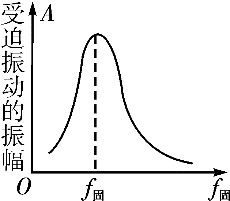
\includegraphics[width=1.04722in,height=0.91528in]{media/image513.png}\end{center}
(2)共振

做受迫振动的物体,它的驱动力的频率与固有频率越接近,其振幅就越大,当二者\_\_相等\_\_时,振幅达到最大,这就是共振现象.共振曲线如图所示.
\subsection{简谐运动的五个特征}

1.动力学特征

F=-kx,``-''表示回复力的方向与位移方向相反,k是比例系数,不一定是弹簧的劲度系数.

2.运动学特征

a=-x,简谐运动的加速度与物体偏离平衡位置的位移成正比而方向相反,为变加速运动,远离平衡位置时,x、F、a、Ep均增大,v、Ek均减小,靠近平衡位置时则相反.

3.运动的周期性特征

相隔T或nT的两个时刻振子处于同一位置且振动状态相同.

4.对称性特征

(1)相隔或()(n为正整数)的两个时刻,振子位置关于平衡位置对称,位移、速度、加速度大小相等,方向相反.

(2)如图所示,振子经过关于平衡位置O对称的两点P、P'(OP=OP')时,速度的大小、动能、势能相等,相对于平衡位置的位移大小相等.

\begin{center}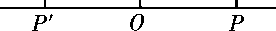
\includegraphics[width=1.25486in,height=0.14167in]{media/image515.png}\end{center}
(3)振子由P到O所用时间等于由O到P'所用时间,即tPO=tOP'. 

(4)振子往复过程中通过同一段路程(如OP段)所用时间相等,即tOP=tPO.

5.能量特征

振动的能量包括动能Ek和势能Ep,简谐运动过程中,系统动能与势能相互转化,系统的机械能守恒.

\begin{center}
\includegraphics[width=0.70764in,height=0.12292in]{media/image37.png}\end{center}
分析简谐运动的技巧

(1)分析简谐运动中各物理量的变化情况时,一定要以位移为桥梁,位移增大时,振动质点的回复力、加速度、势能均增大,速度、动能均减小;反之,则产生相反的变化.另外,各矢量均在其值为零时改变方向.

(2)分析过程中要特别注意简谐运动的周期性和对称性.

{[}例1{]}(多选)一简谐振子沿x轴振动,平衡位置在坐标原点.t=0时刻振子的位移x=-0.1
m;t= s时刻x=0.1 m;t=4 s时刻x=0.1
m.该振子的振幅和周期可能为( AD )

A.0.1 m, s       B.0.1 m,8 s

C.0.2 m, s D.0.2 m,8 s

\subsection{简谐运动的图象}

1.根据简谐运动图象可获取的信息

(1)振幅A、周期T(或频率f)和初相位$\varphi$(如图所示).

\begin{center}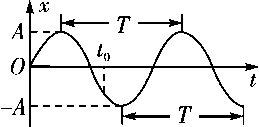
\includegraphics[width=1.17917in,height=0.57569in]{media/image516.png}\end{center}
(2)某时刻振动质点离开平衡位置的位移.

(3)某时刻质点速度的大小和方向:曲线上各点切线的斜率的大小和正负分别表示各时刻质点的速度的大小和速度的方向,速度的方向也可根据下一时刻物体的位移的变化来确定.

(4)某时刻质点的回复力和加速度的方向:回复力总是指向平衡位置,回复力和加速度的方向相同,在图象上总是指向t轴.

(5)某段时间内质点的位移、回复力、加速度、速度、动能和势能的变化情况.

2.利用简谐运动图象理解简谐运动的对称性

\begin{center}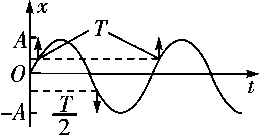
\includegraphics[width=1.17917in,height=0.61319in]{media/image517.png}\end{center}
(1)相隔$\Delta$t=n+T
(n=0,1,2,\ldots)的两个时刻,弹簧振子的位置关于平衡位置对称,位移等大反向,速度也等大反向.

(2)相隔$\Delta$t=nT
(n=0,1,2,\ldots)的两个时刻,弹簧振子在同一位置,位移和速度都相同.

{[}例2{]}一质点做简谐运动,其位移和时间的关系如图所示.

\begin{center}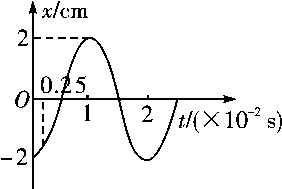
\includegraphics[width=1.28333in,height=0.85833in]{media/image518.png}\end{center}
(1)求t=0.25\ding{54}10-2 s时质点的位移;

(2)在t=1.5\ding{54}10-2 s到t=2\ding{54}10-2
s的振动过程中,质点的位移、回复力、速度、动能、势能如何变化?

(3)在t=0到t=8.5\ding{54}10-2 s时间内,质点的路程、位移各多大?

{[}思维导引{]} (1)看下一时刻位移增加,速度远离时间轴,向正方向运动,否则向负方向运动.加速度方向永远指向时间轴,指向平衡位置.

(2)先增大,后减小,图象上斜率表示速度.

答案 x=-
cm (2)位移变大,回复力变大,速度变小,动能变小,势能变大 (3)34 cm 2
cm

\subsection{受迫振动和共振}

1.自由振动、受迫振动和共振的比较

\begin{longtable}[]{@{}llll@{}}
\toprule
\begin{minipage}[b]{0.22\columnwidth}\raggedright
  振动

项目  \strut
\end{minipage} & \begin{minipage}[b]{0.22\columnwidth}\raggedright
自由振动\strut
\end{minipage} & \begin{minipage}[b]{0.22\columnwidth}\raggedright
受迫振动\strut
\end{minipage} & \begin{minipage}[b]{0.22\columnwidth}\raggedright
共振\strut
\end{minipage}\tabularnewline
\midrule
\endhead
受力情况 & 仅受回复力 & 受驱动力作用 & 受驱动力作用\tabularnewline
\begin{minipage}[t]{0.22\columnwidth}\raggedright
振动周期

或频率 \strut
\end{minipage} & \begin{minipage}[t]{0.22\columnwidth}\raggedright
由系统本身性质决定,即固有周期T0或固有频率f0\strut
\end{minipage} & \begin{minipage}[t]{0.22\columnwidth}\raggedright
由驱动力的周期或频率决定,即T=T驱或f=f驱\strut
\end{minipage} & \begin{minipage}[t]{0.22\columnwidth}\raggedright
T驱=T0或f驱=f0 \strut
\end{minipage}\tabularnewline
振动能量 & 振动物体的机械能不变 & 由产生驱动力的物体提供 &
振动物体获得的能量最大\tabularnewline
常见例子 & 弹簧振子或单摆($\theta \leq 5^\circ$) & 机械工作时底座发生的振动 &
共振筛、声音的共鸣等\tabularnewline
\bottomrule
\end{longtable}

\begin{center}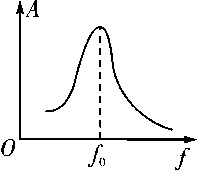
\includegraphics[width=0.89653in,height=0.77361in]{media/image519.png}\end{center}
2.对共振的理解

(1)共振曲线:如图所示,横坐标为驱动力频率f,纵坐标为振幅A.它直观地反映了驱动力频率对某振动系统受迫振动振幅的影响,由图可知,f与f0越接近,振幅A越大;当f=f0时,振幅A最大.

(2)受迫振动中系统能量的转化:受迫振动系统机械能不守恒,系统与外界时刻进行能量交换.

\begin{center}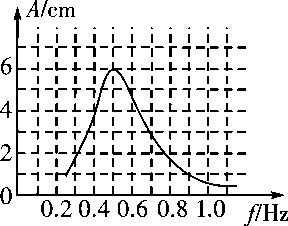
\includegraphics[width=1.31111in,height=1.02847in]{media/image520.png}\end{center}
{[}例3{]}(多选)如图所示是一个单摆做受迫振动时的共振曲线,表示振幅A与驱动力的频率f的关系.下列说法正确的是( BD )

A.摆长约为10 cm

B.摆长约为1 m

C.若增大摆长,共振曲线的``峰''将向右移动

D.若增大摆长,共振曲线的``峰''将向左移动

解析 根据图象可看出单摆的固有频率为0.5 Hz,即周期为2 s.
根据周期公式很容易算出摆长约为1
m,故选项A错误,B正确;若增大摆长,单摆周期将变长,固有频率变小,所以共振曲线的``峰''将向左移动,选项C错误,D正确.

\begin{center}
\includegraphics[width=0.70764in,height=0.12292in]{media/image13.png}\end{center}
(1)无论发生共振与否,受迫振动的频率都等于驱动力的频率,但只有发生共振现象时振幅才能达到最大.

(2)受迫振动系统中的能量转化不再只有系统内部动能和势能的转化,还有驱动力对系统做正功补偿系统因克服阻力而损失的机械能.

\section{机械波}




1.机械波的形成和传播

(1)产生条件

\ding{172}有\_\_波源\_\_.\ding{173}有\_\_介质\_\_,如空气、水、绳子等.

(2)传播特点

\ding{172}传播\_\_振动形式\_\_、能量和信息.

\ding{173}质点不\_\_随波迁移\_\_.

\ding{174}介质中各质点振动频率、振幅、起振方向等都与\_\_波源\_\_相同.

2.机械波的分类

横波和纵波.

3.描述机械波的物理量

(1)波长λ

在波动中,振动相位总是\_\_相同\_\_的两个相邻质点间的距离.用``λ''表示.

(2)频率f

在波动中,介质中各质点的振动频率都是相同的,都等于\_\_波源\_\_的振动频率.

(3)波速v、波长λ和频率f、周期T的关系

公式:v=!!!  \#\#\#=\_\_λf\_\_.

机械波的速度大小由\_\_介质\_\_决定,与机械波的频率无关.

4.波的图象

\begin{center}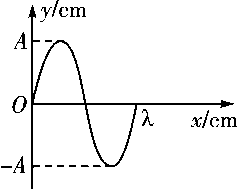
\includegraphics[width=1.07569in,height=0.85833in]{media/image526.png}\end{center}
(1)坐标轴

横轴表示各质点的\_\_平衡\_\_位置,纵轴表示该时刻各质点的\_\_位移\_\_.

(2)图象的意义

表示在波的传播方向上,某时刻各质点离开\_\_平衡\_\_位置的位移.

(3)图象的应用

\ding{172}直接读取\_\_振幅A\_\_和\_\_波长λ\_\_,以及该时刻各质点的位移.

\ding{173}确定某时刻各质点加速度的\_\_方向\_\_,并能比较其大小.

\ding{174}结合波的传播方向可确定各质点的振动\_\_方向\_\_或由各质点的振动方向确定波的\_\_传播方向\_\_.

5.波的干涉和衍射现象 多普勒效应

(1)波的干涉和衍射

\begin{longtable}[]{@{}lll@{}}
\toprule
& 波的干涉 & 波的衍射\tabularnewline
\midrule
\endhead
条件 & 两列波的频率必须\_\_相同\_\_,相位差保持不变 &
产生明显衍射的条件:障碍物或孔的\_\_尺寸\_\_比波长小或相差不多\tabularnewline
现象 & 形成加强区和减弱区相互隔开的稳定的\_\_干涉图样\_\_ &
波能够\_\_绕过障碍物\_\_或孔继续向前传播\tabularnewline
\bottomrule
\end{longtable}

(2)多普勒效应

\ding{172}条件:声源和观察者之间有\_\_相对运动\_\_;

\ding{173}现象:观察者感到\_\_频率\_\_发生变化;

\ding{174}实质:声源频率不变,观察者接收到的\_\_频率\_\_变化.
\subsection{对波动图象的理解与应用}

1.波的图象描述的是在波的传播方向上,介质中的各个质点在某一时刻相对各自平衡位置的位移.

2.在波的传播方向上,当两质点平衡位置间的距离为nλ
(n=1,2,3,\ldots)时,它们的振动步调总相同;当两质点平衡位置间的距离为(2n+1)
(n=0,1,2,3,\ldots)时,它们的振动步调总相反.

3.波源质点的起振方向决定了它后面的质点的起振方向,各质点的起振方向与波源的起振方向相同.

\begin{center}
\includegraphics[width=0.70764in,height=0.12292in]{media/image37.png}\end{center}
波的传播方向与质点振动方向的互判方法

\begin{longtable}[]{@{}lll@{}}
\toprule
& 内容 & 图象\tabularnewline
\midrule
\endhead
``上下坡''法 &
沿波的传播方向,``上坡''时质点向下振动,``下坡''时质点向上振动 &
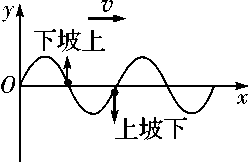
\includegraphics[width=1.13194in,height=0.73611in]{media/image528.png}\tabularnewline
``同侧''法 & 波形图上某点表示传播方向和振动方向的箭头在图线同侧 &
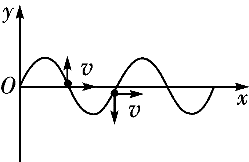
\includegraphics[width=1.13194in,height=0.73611in]{media/image529.png}\tabularnewline
``微平移''法 &
将波形沿传播方向进行微小的平移,再由对应同一x坐标的两波形曲线上的点来判断振动方向
&
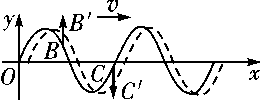
\includegraphics[width=1.18889in,height=0.45278in]{media/image530.png}\tabularnewline
\bottomrule
\end{longtable}

{[}例1{]}(多选)一列沿x轴正方向传播的简谐机械横波,波速为4
m/s.某时刻波形如图所示,下列说法正确的是( DE )

\begin{center}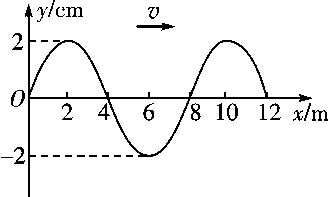
\includegraphics[width=1.49028in,height=0.89653in]{media/image531.png}\end{center}
A.这列波的振幅为4 cm

B.这列波的周期为1 s

C.此时x=4 m处质点沿y轴负方向运动

D.此时x=4 m处质点的加速度为零

E.从此时开始5 s后x=4 m处的质点沿y轴负方向运动

解析 由图象可知波的振幅为2 cm,选项A错误;由T=可知T=2
s,选项B错误;由于波向右传播,x=4
m处的质点向上运动,加速度为零,选项C错误,D正确;t=
T时,质点振动方向相反,故x=4 m处的质点沿y轴负方向运动,选项E正确.

\subsection{振动图象和波动图象的综合应用}

振动图象与波动图象的比较

\begin{longtable}[]{@{}lll@{}}
\toprule
& 振动图象 & 波动图象\tabularnewline
\midrule
\endhead
研究对象 & 一振动质点 & 沿波传播方向所有质点\tabularnewline
研究内容 & 一质点位移随时间变化规律 &
某时刻所有质点的空间分布规律\tabularnewline
图象 &
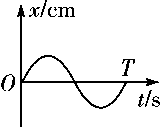
\includegraphics[width=0.72639in,height=0.57569in]{media/image532.png} &
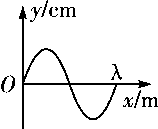
\includegraphics[width=0.71667in,height=0.58472in]{media/image533.png}\tabularnewline
物理意义 & 表示同一质点在各时刻的位移 &
表示某时刻各质点的位移\tabularnewline
\begin{minipage}[t]{0.30\columnwidth}\raggedright
图象信息\strut
\end{minipage} & \begin{minipage}[t]{0.30\columnwidth}\raggedright
(1)质点振动周期

(2)质点振幅

(3)各时刻质点位移

(4)各时刻速度、加速度方向\strut
\end{minipage} & \begin{minipage}[t]{0.30\columnwidth}\raggedright
(1)波长、振幅

(2)任意一质点此刻的位移

(3)任意一质点在该时刻加速度方向

(4)传播方向、振动方向的互判\strut
\end{minipage}\tabularnewline
形象比喻 & 记录着一个人一段时间内活动的录像带 &
记录着许多人某时刻动作、表情的集体照片\tabularnewline
图象变化 & 随时间推移图象延续,但已有形状不变 &
随时间推移,波形沿传播方向平移\tabularnewline
一完整曲线占横坐标距离 & 表示一个周期 & 表示一个波长\tabularnewline
\bottomrule
\end{longtable}

\begin{center}
\includegraphics[width=0.70764in,height=0.12292in]{media/image37.png}\end{center}
巧解波动图象与振动图象综合类问题

(1)分清振动图象与波动图象.只要看清横坐标即可,横坐标为x则为波动图象,横坐标为t则为振动图象.

(2)看清横、纵坐标的单位,注意单位前的数量级.

(3)找准波动图象对应的质点.

(4)找准振动图象对应的时刻.

{[}例2{]}(多选)图甲为一列简谐横波在t=0.10
s时刻的波形图,P是平衡位置在x=1.0 m处的质点,Q是平衡位置在x=4.0
m处的质点;图乙为质点Q的振动图象.下列说法正确的是( BCE )

\begin{center}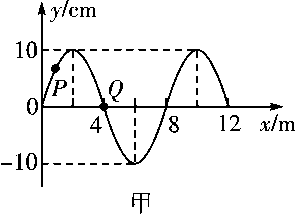
\includegraphics[width=1.33958in,height=0.97153in]{media/image534.png}\end{center}

\begin{center}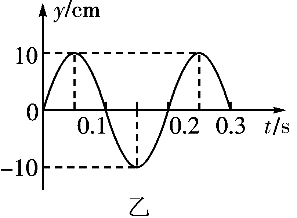
\includegraphics[width=1.34931in,height=0.99028in]{media/image535.png}\end{center}
A.在t=0.10 s时,质点Q向y轴正方向运动

B.在t=0.25 s时,质点P的加速度方向与y轴正方向相同

C.从t=0.10 s到t=0.25 s,该波沿x轴负方向传播了6 m

D.从t=0.10 s到t=0.25 s,质点P通过的路程为30 cm

E.质点Q简谐运动的表达式为y=0.10sin 10πt (国际单位制)

\begin{center}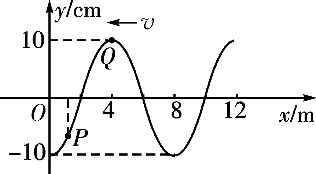
\includegraphics[width=1.43403in,height=0.79236in]{media/image536.png}\end{center}
\subsection{波的多解问题}

1.造成波动问题多解的主要因素

(1)周期性

\ding{172}时间周期性:时间间隔$\Delta$t与周期T的关系不明确;

\ding{173}空间周期性:波传播距离$\Delta$x与波长λ的关系不明确.

(2)双向性

\ding{172}传播方向双向性:波的传播方向不确定;

\ding{173}振动方向双向性:质点振动方向不确定.

(3)波形的隐含性形成多解

在波动问题中,往往只给出完整波形的一部分,或给出几个特殊点,而其余信息均处于隐含状态.这样,波形就有多种情况,形成波动问题的多解性.

2.解决波的多解问题的思路

一般采用从特殊到一般的思维方法,即找出一个周期内满足条件的关系$\Delta$t或$\Delta$x,若此关系为时间,则t=nT+$\Delta$t
(n=0,1,2,\ldots);若此关系为距离,则x=nλ+$\Delta$x(n=0,1,2,\ldots).

\begin{center}
\includegraphics[width=0.70764in,height=0.12292in]{media/image37.png}\end{center}
求解波的多解问题的一般步骤

(1)根据初、末两时刻的波形图确定传播距离与波长的关系通式.

(2)根据题设条件判断是唯一解还是多解.

(3)根据波速公式v=或v==λf求波速.

{[}例3{]}(2017·湖南长沙长郡中学月考)一列简谐横波图象如图所示,t1时刻的波形如图中实线所示,t2时刻的波形如图中虚线所示,已知$\Delta$t=t2-t1=0.5
s.

\begin{center}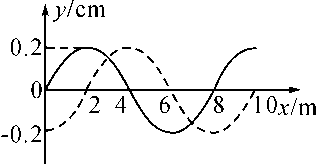
\includegraphics[width=1.44306in,height=0.74514in]{media/image537.png}\end{center}
(1)求这列波的可能的波速表达式;

(2)若波向左传播,且3T\textless $\Delta$t\textless4T,则波速为多大?

(3)若波速v=68 m/s,则波向哪个方向传播?

{[}思维导引{]}本题产生多解的原因:

一是由于波的传播方向的双向性;

二是由于波的空间周期性.

答案 (1)见解析 (2)60 m/s (3)向右

\subsection{波的干涉和衍射 多普勒效应}

1.波的干涉现象中加强点、减弱点的两种判断方法

(1)公式法

某质点的振动是加强还是减弱,取决于该点到两相干波源的距离之差$\Delta$r.

\ding{172}当两波源振动步调一致时

若$\Delta$r=nλ (n=0,1,2,\ldots),则振动加强;

若$\Delta$r=(2n+1) (n=0,1,2,\ldots),则振动减弱.

\ding{172}当两波源振动步调相反时

若$\Delta$r=(2n+1) (n=0,1,2,\ldots),则振动加强;

若$\Delta$r=nλ (n=0,1,2,\ldots),则振动减弱.

(2)图象法

在某时刻波的干涉的波形图上,波峰与波峰(或波谷与波谷)的交点,一定是加强点,而波峰与波谷的交点一定是减弱点,各加强点或减弱点各自连接而成以两波源为中心向外辐射的连线,形成加强线和减弱线,两种线互相间隔,加强点与减弱点之间各质点的振幅介于加强点与减弱点的振幅之间.

2.多普勒效应

(1)产生条件:波源与观察者之间有相对运动.

(2)现象:两者相互靠近时,感觉波的频率升高;两者相互远离时,感觉波的频率降低.

{[}例4{]}(多选)如图所示,S1、S2是两个相干波源,它们振动同步且振幅相同.实线和虚线分别表示在某一时刻它们所发出的波的波峰和波谷.图中所标的a、b、c、d四点中d点到两波源距离相等,下列说法中正确的有
( BC )

\begin{center}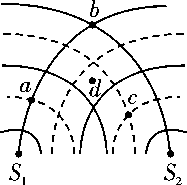
\includegraphics[width=0.84931in,height=0.83958in]{media/image538.png}\end{center}
A.该时刻a质点振动最弱,b、c质点振动最强,d质点振动既不是最强也不是最弱

B.该时刻a质点振动最弱,b、c、d质点振动都最强

C.a质点的振动始终是最弱的,b、c、d质点的振动始终是最强的

D.再过后的时刻,a、b、c三个质点都将处于各自的平衡位置,因此振动最弱

{[}例5{]}(多选)如图甲所示,男同学站立不动吹口哨,一位女同学坐在秋千上来回摆动,据图乙.下列关于女同学的感受的说法正确的是( AD )

\begin{center}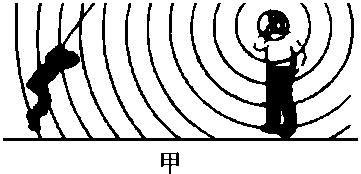
\includegraphics[width=1.64167in,height=0.79236in]{media/image539.png}\end{center}

\begin{center}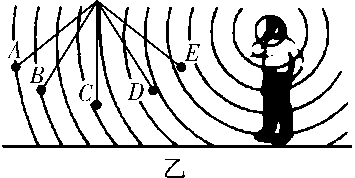
\includegraphics[width=1.61319in,height=0.81111in]{media/image540.png}\end{center}
A.女同学从A向B运动过程中,她感觉哨声音调变高

B.女同学从E向D运动过程中,她感觉哨声音调变高

C.女同学在点C向右运动时,她感觉哨声音调不变

D.女同学在点C向左运动时,她感觉哨声音调变低

\section{光的折射 全反射}



1.光的折射定律 折射率

(1)折射现象

光从一种介质斜射进入另一种介质时传播方向发生\_\_改变\_\_的现象,如图所示.

\begin{center}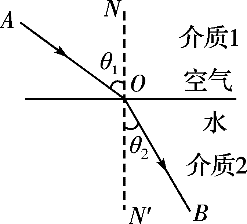
\includegraphics[width=1.12292in,height=1.01875in]{media/image545.png}\end{center}
(2)折射定律

\ding{172}内容:折射光线与入射光线、法线处在同一平面内,折射光线与入射光线分别位于法线的\_\_两侧\_\_;入射角的正弦与折射角的正弦成\_\_正比\_\_.

(2)表达式:=n12,式中n12是比例常数.

(3)折射率

\ding{172}物理意义:折射率反映介质的光学特征,折射率大,说明光线从真空射入到该介质时\_\_偏折大\_\_,反之偏折小.

\ding{173}定义式:n=,不能说n与sin $\theta$1成正比,与sin
$\theta$2成反比.折射率由介质本身的光学性质和光的\_\_频率\_\_决定.

\ding{174}计算公式:n=.

2.全反射 光导纤维

(1)光密介质与光疏介质

\begin{longtable}[]{@{}lll@{}}
\toprule
\begin{minipage}[b]{0.30\columnwidth}\raggedright
   介质

项目   \strut
\end{minipage} & \begin{minipage}[b]{0.30\columnwidth}\raggedright
光密介质\strut
\end{minipage} & \begin{minipage}[b]{0.30\columnwidth}\raggedright
光疏介质\strut
\end{minipage}\tabularnewline
\midrule
\endhead
折射率 & 大 & 小\tabularnewline
光速 & 小 & 大\tabularnewline
\begin{minipage}[t]{0.30\columnwidth}\raggedright
相对性\strut
\end{minipage} & \begin{minipage}[t]{0.30\columnwidth}\raggedright
若n甲\textgreater n乙,则甲是\_\_光密\_\_介质

若n甲\textless n乙,则甲是\_\_光疏\_\_介质\strut
\end{minipage} & \begin{minipage}[t]{0.30\columnwidth}\raggedright
\strut
\end{minipage}\tabularnewline
\bottomrule
\end{longtable}

(2)全反射

\ding{172}定义:光从光密介质射入光疏介质,当入射角增大到某一角度时,折射光线将\_\_消失\_\_,只剩下反射光线的现象.

\ding{173}条件:

a.光从光密介质射向光疏介质.

b.入射角\_\_大于或等于\_\_临界角.

\ding{174}临界角:折射角等于$90^\circ$时的入射角.若光从光密介质(折射率为n)射向真空或空气时,发生全反射的临界角为C,则sin
C=.介质的折射率越大,发生全反射的临界角越小.

(3)光导纤维

光导纤维的原理是利用光的全反射.

\begin{center}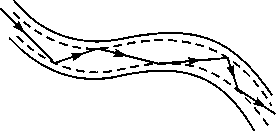
\includegraphics[width=1.25486in,height=0.59444in]{media/image546.png}\end{center}
\subsection{对折射率的理解}

(1)公式n=中,不论光是从真空射入介质,还是从介质射入真空,$\theta$1总是真空中的光线与法线间的夹角,$\theta$2总是介质中的光线与法线间的夹角.

(2)折射率由介质本身性质决定,与入射角的大小无关.

(3)折射率与介质的密度没有关系,光密介质不是指密度大的介质.

(4)折射率的大小不仅与介质本身有关,还与光的频率有关.

同一种介质中,频率越大的色光折射率越大,光在介质中的传播速度越小.

(5)同一种色光,在不同介质中虽然波速、波长不同,但频率相同.

2.光路的可逆性

在光的折射现象中,光路是可逆的.如果让光线逆着原来的折射光线射到界面上,光线就会逆着原来的入射光线发生折射.

\begin{center}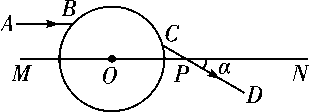
\includegraphics[width=1.40556in,height=0.50972in]{media/image547.png}\end{center}
{[}例1{]}(2017·重庆诊断性测试)如图所示,一透明球体置于空气中,球半径R=10
cm,折射率n=,MN是一条通过球心的直线,单色细光束AB平行于MN射向球体,B为入射点,AB与MN间距为5
cm,CD为出射光线.

(1)补全光路图并求出光从B点传到C点的时间;

(2)求CD与MN所成的角$\alpha$.

\begin{center}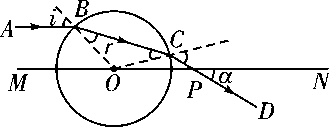
\includegraphics[width=1.5in,height=0.57569in]{media/image548.png}\end{center}
答案 (1)见解析 (2)$30^\circ$

\begin{center}
\includegraphics[width=0.70764in,height=0.12292in]{media/image13.png}\end{center}
应用光的折射定律解题的一般思路

(1)根据入射角、折射角及反射角之间的关系,作出比较完整的光路圈.

(2)充分利用光路图中的几何关系,确定各角之间的联系,根据折射定律求解相关的物理量:折射角、折射率等.

(3)注意在折射现象中,光路是可逆的.

\subsection{光的折射与全反射的综合应用}

1.光密介质和光疏介质是相对而言的.同一种介质,相对于其他不同的介质,可能是光密介质,也可能是光疏介质.

2.如果光线从光疏介质进入光密介质,则无论入射角多大,都不会发生全反射现象.

3.在光的折射和全反射现象中,均遵循光的反射定律,光路均是可逆的.

4.当光射到两种介质的界面上时,往往同时发生光的折射和反射现象,但在全反射现象中,只发生反射,不发生折射.

\begin{center}
\includegraphics[width=0.70764in,height=0.12292in]{media/image13.png}\end{center}
解决全反射问题的一般方法

(1)确定光是从光密介质进入光疏介质.

(2)应用sin C=确定临界角.

(3)根据题设条件,判定光在传播时是否发生全反射.

(4)如发生全反射,画出入射角等于临界角时的临界光路图.

(5)运用几何关系或三角函数关系以及反射定律等进行分析、判断、计算.

{[}例2{]}(2017·全国卷Ⅰ)如图,一玻璃工件的上半部是半径为R的半球体,O点为球心;下半部是半径为R、高为2R的圆柱体,圆柱体底面镀有反射膜.有一平行于中心轴OC的光线从半球面射入,该光线与OC之间的距离为0.6R.已知最后从半球面射出的光线恰好与入射光线平行(不考虑多次反射).求该玻璃的折射率.

\begin{center}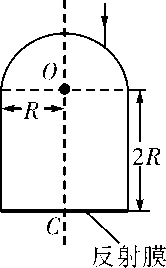
\includegraphics[width=0.75486in,height=1.21667in]{media/image549.png}\end{center}
答案 1.43

\subsection{光的色散}

1.光的色散:把复色光分解为单色光的现象叫做光的色散.白光通过棱镜后,被分解为红、橙、黄、绿、蓝、靛和紫七种颜色(如图).

\begin{center}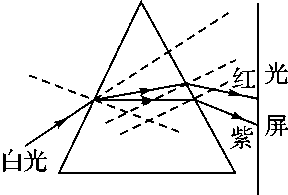
\includegraphics[width=1.31111in,height=0.88681in]{media/image550.png}\end{center}
2.正确理解光的色散

(1)光的颜色由光的频率决定.

(2)各种色光的比较

\begin{longtable}[]{@{}ll@{}}
\toprule
颜色 & 红橙黄绿青蓝紫\tabularnewline
\midrule
\endhead
频率ν & 低$\rightarrow$高\tabularnewline
同一介质中的折射率 & 小$\rightarrow$大\tabularnewline
同一介质中速度 & 大$\rightarrow$小\tabularnewline
波长 & 大$\rightarrow$小\tabularnewline
临界角 & 大$\rightarrow$小\tabularnewline
通过棱镜的偏折角 & 小$\rightarrow$大\tabularnewline
\bottomrule
\end{longtable}

{[}例3{]}(多选)如图所示,一束光沿半径方向射向一块半圆柱形玻璃砖,在玻璃砖底面上的入射角为$\theta$,经折射后射出a、b两束光线.则( ABD )

\begin{center}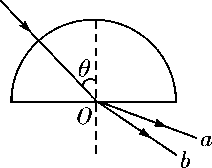
\includegraphics[width=0.9625in,height=0.76389in]{media/image551.png}\end{center}
A.在玻璃中,a光的传播速度小于b光的传播速度

B.在真空中,a光的波长小于b光的波长

C.玻璃砖对a光的折射率小于对b光的折射率

D.若改变光束的入射方向使$\theta$角逐渐变大,则折射光线a首先消失

E.分别用a、b光在同一个双缝干涉实验装置上做实验,a光的干涉条纹间距大于b光的干涉条纹间距

解析 通过光路图可看出,折射后a光的偏折程度大于b光的偏折程度,玻璃砖对a光的折射率大于b光的折射率,选项C错误;a光的频率大于b光的频率,波长小于b光的波长,选项B正确;由n=知,在玻璃中,a光的传播速度小于b光的传播速度,选项A正确;入射角增大时,折射率大的光线首先发生全反射,a光首先消失,选项D正确;做双缝干涉实验时,根据$\Delta$x=λ得a光的干涉条纹间距小于b光的干涉条纹间距,选项E错误.

\section{光的波动性 电磁波和相对论}



1.光的干涉

(1)定义:在两列光波叠加的区域,某些区域相互加强,出现\_\_亮\_\_条纹,某些区域相互减弱,出现\_\_暗\_\_条纹,且加强区域和减弱区域相互间隔的现象.

(2)条件:两束光的频率\_\_相同\_\_、相位差恒定.

(3)双缝干涉图样特点:单色光照射时形成明暗相间的等间距的干涉条纹;白光照射时,中央为\_\_白色亮\_\_条纹,其余为\_\_彩色\_\_条纹.

2.光的衍射

(1)发生明显衍射的条件

只有当障碍物的尺寸与光的波长\_\_相差不多\_\_,甚至比光的波长\_\_还小\_\_的时候,衍射现象才会明显.

(2)衍射条纹的特点

\ding{172}单缝衍射:单色光的衍射图样为中间\_\_宽且亮\_\_的单色条纹,两侧是\_\_明暗相间\_\_的条纹,条纹宽度比中央窄且暗;白光的衍射图样为中间宽且亮的白条纹,两侧是渐窄且暗的彩色条纹.

\begin{center}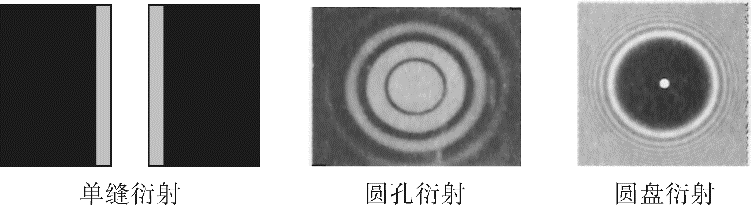
\includegraphics[width=3.41528in,height=0.93403in]{media/image557.png}\end{center}
\ding{173}圆孔衍射:明暗相间的\_\_不等距\_\_圆环.如图所示.

\ding{174}泊松亮斑(圆盘衍射):当光照到\_\_不透明\_\_(选填``透明''或``不透明'')的半径很小的小圆盘上时,在圆盘的阴影中心出现\_\_亮斑\_\_(在阴影外还有不等间距的明暗相间的圆环).如图所示.

3.光的偏振

(1)自然光:包含着在垂直于传播方向上沿\_\_一切方向\_\_振动的光,而且沿着各个方向振动的光波的强度都相同.

(2)偏振光:在垂直于光的传播方向的平面上,只沿着某个\_\_特定\_\_的方向振动的光.

(3)偏振光的形成:

\ding{172}让自然光通过\_\_偏振片\_\_形成偏振光.

\ding{173}让自然光在两种介质的界面发生反射和\_\_折射\_\_,反射光和折射光可以成为部分偏振光或完全偏振光.

(4)光的偏振现象说明光是一种\_\_横\_\_波.

4.电磁波的产生

(1)麦克斯韦电磁场理论

变化的磁场产生\_\_电场\_\_,变化的电场产生\_\_磁场\_\_.

(2)电磁场

变化的电场和变化的磁场总是相互联系成为一个完整的整体,这就是电磁场.

(3)电磁波

电磁场(电磁能量)由近及远地向周围传播形成电磁波.

\ding{172}电磁波是横波,在空间传播\_\_不需要\_\_介质;

\ding{173}真空中电磁波的速度为\_\_3.0\ding{54}108\_\_m/s;

\ding{174}v=λf对电磁波\_\_同样适用\_\_;

\ding{175}电磁波能产生反射、折射、\_\_干涉\_\_和衍射等现象.

5.电磁波的发射和接收

(1)发射电磁波的条件

\ding{172}要有足够高的\_\_振荡频率\_\_;

\ding{173}电路必须\_\_开放\_\_,使振荡电路的电场和磁场分散到尽可能大的空间.

(2)调制有\_\_调幅\_\_和调频两种方式,解调是调制的逆过程.

(3)电磁波谱

\ding{172}定义:按电磁波的波长从长到短分布是\_\_无线电波\_\_、红外线、可见光、紫外线、X射线和γ射线,形成电磁波谱;递变规律:直线传播能力增强,衍射能力减弱.

\ding{173}电磁波谱的特性、应用

\begin{longtable}[]{@{}lll@{}}
\toprule
电磁波谱 & 特性 & 应用\tabularnewline
\midrule
\endhead
红外线 & \_\_热效应\_\_ & 红外线遥感\tabularnewline
\begin{minipage}[t]{0.30\columnwidth}\raggedright
紫外线\strut
\end{minipage} & \begin{minipage}[t]{0.30\columnwidth}\raggedright
化学效应、\_\_荧光效应\_\_、

能杀菌\strut
\end{minipage} & \begin{minipage}[t]{0.30\columnwidth}\raggedright
医用消毒、防伪\strut
\end{minipage}\tabularnewline
X射线 & 贯穿性强 & 检查、医用透视\tabularnewline
γ射线 & 贯穿本领最强 & 工业探伤、医用治疗\tabularnewline
\bottomrule
\end{longtable}

6.狭义相对论

(1)狭义相对论的两个基本假设

\ding{172}狭义相对性原理:在不同的惯性参考系中,一切物理规律都是\_\_相同\_\_的.

\ding{173}光速不变原理:真空中的光速在不同的惯性参考系中都是\_\_相同\_\_的,光速与光源、观测者间的相对运动没有关系.

(2)相对论的质速关系

\ding{172}物体的质量随物体速度的增加而增大,物体以速度v运动时的质量m与静止时的质量m0之间有如下关系:m=!!! () \#\#\#.

\ding{173}物体运动时的质量m总要\_\_大于\_\_静止时的质量m0.

7.相对论质能关系

用m表示物体的质量,E表示它具有的能量,则爱因斯坦质能方程为:E=\_\_mc2\_\_.
\subsection{光的干涉、衍射和偏振}

1.光的双缝干涉现象

(1)明暗条纹的判断方法

\ding{172}如图所示,光源S1、S2发出的光到屏上P点的路程差r2-r1=kλ
(k=0,1,2,\ldots)时,光屏上出现明条纹.

\begin{center}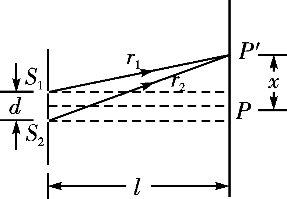
\includegraphics[width=1.30208in,height=0.90556in]{media/image558.png}\end{center}

\ding{173}光的路程差r2-r1=(2k+1)
(k=0,1,2,\ldots)时,光屏上出现暗条纹.

(2)条纹间距:$\Delta$x=λ,其中L是双缝到光屏的距离,d是双缝间的距离,λ是光波的波长.

2.对光的衍射的理解

(1)干涉和衍射是波的特征,波长越长,干涉和衍射现象越明显.在任何情况下都可以发生衍射现象,只是明显与不明显的差别.

(2)衍射现象说明``光沿直线传播''只是一种特殊情况,只有在光的波长比障碍物小得多时,光才可以看做是沿直线传播的.

3.单缝衍射与双缝干涉的比较

\begin{longtable}[]{@{}llll@{}}
\toprule
\begin{minipage}[b]{0.22\columnwidth}\raggedright
   两种现象

比较项目   \strut
\end{minipage} & \begin{minipage}[b]{0.22\columnwidth}\raggedright
单缝衍射\strut
\end{minipage} & \begin{minipage}[b]{0.22\columnwidth}\raggedright
双缝干涉\strut
\end{minipage} & \begin{minipage}[b]{0.22\columnwidth}\raggedright
\strut
\end{minipage}\tabularnewline
\midrule
\endhead
\begin{minipage}[t]{0.22\columnwidth}\raggedright
不

同

点\strut
\end{minipage} & \begin{minipage}[t]{0.22\columnwidth}\raggedright
条纹宽度\strut
\end{minipage} & \begin{minipage}[t]{0.22\columnwidth}\raggedright
条纹宽度不等,中央最宽\strut
\end{minipage} & \begin{minipage}[t]{0.22\columnwidth}\raggedright
条纹宽度相等\strut
\end{minipage}\tabularnewline
& 条纹间距 & 各相邻条纹间距不等 & 各相邻条纹等间距\tabularnewline
& 亮度情况 & 中央条纹最亮,两边变暗 &
条纹清晰,亮度基本相等\tabularnewline
相同点 & 干涉、衍射都是波特有的现象;干涉、衍射都有明暗相间的条纹 &
&\tabularnewline
\bottomrule
\end{longtable}

4.干涉与衍射的本质

光的干涉条纹和衍射条纹都是光波叠加的结果,从本质上讲,衍射条纹的形成与干涉条纹的形成具有相似的原理.在衍射现象中,可以认为从单缝通过两列或多列频率相同的光波,它们在屏上叠加形成单缝衍射条纹.

5.光的偏振

(1)自然光与偏振光的比较

\begin{longtable}[]{@{}lll@{}}
\toprule
类别 & 自然光(非偏振光) & 偏振光\tabularnewline
\midrule
\endhead
光的来源 & 从普通光源发出的光 & 自然光通过起偏器后的光\tabularnewline
光的振动方向 &
在垂直于光的传播方向的平面内,光振动沿任意方向,且沿各个方向振动的光的强度相同
& 在垂直于光的传播方向的平面内,光振动沿特定方向\tabularnewline
\bottomrule
\end{longtable}

(2)偏振光的应用:加偏振滤光片的照相机镜头、液晶显示器、立体电影、消除车灯眩光等。

{[}例1{]}如图所示为条纹总宽度相同的4种明暗相间的条纹,其中有两种是红光、蓝光各自通过同一个双缝干涉仪器形成的干涉图样,还有两种是黄光、紫光各自通过同一个单缝形成的衍射图样(灰黑色部分表示亮纹).则图中从左向右排列,亮条纹的颜色依次是( B )

\begin{center}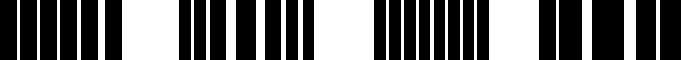
\includegraphics[width=3.09444in,height=0.27361in]{media/image559.png}\end{center}
A.红黄蓝紫 B.红紫蓝黄

C.蓝紫红黄 D.蓝黄红紫

\subsection{薄膜干涉现象的理解}

1.如图所示,竖直的肥皂薄膜,由于重力的作用,形成上薄下厚的楔形.

\begin{center}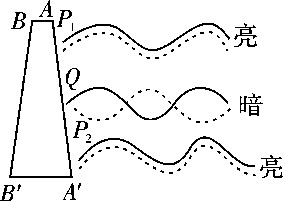
\includegraphics[width=1.28333in,height=0.91528in]{media/image560.png}\end{center}
2.光照射到薄膜上时,在膜的前表面AA'和后表面BB'分别反射出来,相互叠加,发生干涉.

3.原理分析

(1)单色光

\ding{172}在P1、P2处,两个表面反射回来的两列光波的路程差$\Delta$r等于薄膜中波长的整数倍.

$\Delta$r=nλ (n=1,2,3,\ldots),薄膜上出现明条纹.

\ding{173}在Q处,两列反射回来的光波的路程差$\Delta$r等于半波长的奇数倍.$\Delta$r=(2n+1)
(n=0,1,2,3,\ldots),薄膜上出现暗条纹.

(2)白光:薄膜上出现水平彩色条纹.

4.薄膜干涉的应用

干涉法检查平面如图所示,两板之间形成一楔形空气膜,用单色光从上向下照射,如果被检平面是平整光滑的,我们会观察到平行且等间距的明暗相间的条纹;若被检平面不平整,则干涉条纹发生弯曲.

\begin{center}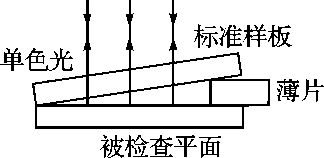
\includegraphics[width=1.47153in,height=0.71667in]{media/image561.png}\end{center}
{[}例2{]}(多选)把一平行玻璃板压在另一个平行玻璃板上,一端用薄片垫起,构成空气劈尖,让单色光从上方射入,如图所示.这时可以看到明暗相间的条纹.下面关于条纹的说法中正确的是( AC )

\begin{center}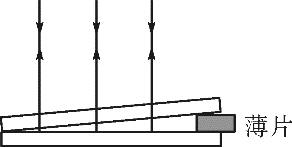
\includegraphics[width=1.32986in,height=0.67014in]{media/image562.png}\end{center}
A.干涉条纹是光在空气劈尖膜的前后两表面反射形成的两列光波叠加的结果

B.干涉条纹中的暗条纹是上述两列反射光的波谷与波谷叠加的结果

C.将上玻璃板平行上移,条纹向着劈尖移动

D.观察薄膜干涉条纹时,应在入射光的另一侧

解析 根据薄膜干涉的产生原理,上述现象是由空气劈尖膜前后表面反射的两列光叠加而成,当波峰与波峰、波谷与波谷相遇叠加时,振动加强,形成亮条纹,所以选项A正确,B错误.因相干光是反射光,故观察薄膜干涉时,应在入射光的同一侧,故选项D错误.条纹的位置与空气劈尖膜的厚度是对应的,当上玻璃板平行上移时,同一厚度的空气劈尖膜向劈尖移动,故条纹向着劈尖移动,故选项C正确.

\subsection{电磁场和电磁波}

1.电磁场

如果在空间某区域中有周期性变化的电场,那么这个变化的电场就在它周围空间产生周期性变化的磁场;这个变化的磁场又在它周围空间产生新的周期性变化的电场\ldots\ldots 变化的电场和变化的磁场是相互联系着的,形成不可分割的统一体,这就是电磁场.

2.电磁波的波速、波长与频率的关系:c=λf,λ=.

\ding{172}同一种电磁波在不同介质中传播时,频率不变(频率由波源决定),波速、波长发生改变.在介质中的速度都比在真空中速度小.

\ding{173}不同电磁波在同一种介质中传播时,传播速度不同,频率越高波速越小,频率越低波速越大.

3.电磁波与机械波的比较

\begin{longtable}[]{@{}lll@{}}
\toprule
& 机械波 & 电磁波\tabularnewline
\midrule
\endhead
研究对象 & 研究力学现象 & 研究电磁现象\tabularnewline
周期性变化的物理量 & 位移随时间和空间做周期性变化 &
电场E和磁感应强度B随时间和空间做周期性变化\tabularnewline
传播 & 传播需要介质,波速与介质有关,与频率无关 &
传播无需介质,在真空中波速总是c,在介质中传播时,波速与介质及频率都有关系\tabularnewline
产生 & 由质点(波源)的振动产生 &
由周期性变化的电流(电磁振荡)激发\tabularnewline
纵波还是横波 & 可以是纵波也可以是横波 & 横波\tabularnewline
联系 &
都具有波的一切特性,例如干涉、衍射、反射、折射等性质,它们的波速、波长与频率的关系都是v=λf,都能传播能量
&\tabularnewline
\bottomrule
\end{longtable}

{[}例3{]}(多选)关于电磁场和电磁波,下列叙述中正确的是( CD )

A.恒定的电场能够产生电磁波

B.电磁波的传播需要介质

C.电磁波从一种介质进入另一种介质,频率不变

D.电磁波在传播过程中也传递了能量

解析 由麦克斯韦电磁场理论可知,只有非均匀变化的电场、磁场能产生电磁波,选项A错误;电磁波的传播不需要介质,选项B错误;电磁波与机械波一样,在传播过程中频率不变,选项C正确;电磁波传播电磁振荡的运动形式和能量,选项D正确.

\subsection{狭义相对论}

1.对``同时''的相对性的理解:``同时''具有相对性,即在同一个惯性系中不同地点同时发生的两个事件,在另一个惯性系中观察就不一定是同时发生的.

2.对``长度的相对性''的理解:狭义相对论中的长度公式:l=l0中,l0是相对于杆静止的观察者测出的杆的长度,而l可认为杆沿杆的长度方向以速度v运动时,静止的观察者测量的长度,或观察者沿杆的长度方向以速度v运动时测出的杆的长度.

3.对``时间间隔的相对性''的理解:时间间隔的相对性公式:$\Delta$t=中$\Delta$τ是相对事件发生地静止的观察者测量同一地点的两个事件发生的时间间隔,而$\Delta$t则是相对于事件发生地以速度v运动的观察者测量同一地点的同样两个事件发生的时间间隔.也就是说:在相对运动的参考系中观测,事件变化过程的时间间隔变大了,这叫做狭义相对论中的时间膨胀.(动钟变慢)

4.对相对论速度变换公式的理解:速度变换公式u=.式中u是物体相对静止参考系的速度,v是运动参考系相对静止参考系的速度,u'是物体相对运动参考系的速度.(u'与v同向取正值,反之取负值)

{[}例4{]}---艘太空飞船静止时的长度为30m,他以0.6c(c为光速)的速度沿长度方向飞行经过地球,下列说法正确的是( B )

A.飞船上的观测者测得该飞船的长度小于30 m

B.地球上的观测者测得该飞船的长度小于30 m

C.飞船上的观测者测得地球上发来的光信号速度小于c

D.地球上的观测者测得飞船上发来的光信号速度小于c

解析 飞船上的观察者相对飞船是静止的,测得飞船长度为静止长度30
m,选项A错误;地球上的观察者相对飞船的速度为0.6
c,测得飞船的长度l=l0()=0.8 l0=24
m,选项B正确;由光速不变原理知光信号的速度与参考系无关,选项C、D皆错误.

\begin{center}
\includegraphics[width=0.70764in,height=0.12292in]{media/image37.png}\end{center}
\begin{center}
  \textbf{狭义相对论问题的求解技巧}
\end{center}

(1)解决``同时''的相对性问题,可从三个方面入手:

\ding{172}令观察者静止,判断被观察者因相对运动而引起的位置变化.

\ding{173}结合光速不变原理,分析光传播到两个事件所用的时间.

\ding{174}光先传播到的事件先发生,光后传播到的事件后发生.

(2)``动尺缩短''是沿运动方向上的长度比其相对静止时测量的长度要短一些,在垂直于运动方向上的长度没有变化.

(3)``动钟变慢''是两个不同惯性系进行时间比较的结果,也是相对的,即两个惯性系中的观察者都发现对方的钟变慢了.
